\chapter{Additional information regarding the impact of COVID-19 lockdowns (\cref{ch:lockdown})}
\label{app:lockdown} 

\section{Online Questionnaire}

\begin{table}[!ht]
\centering
\caption{Questionnaire deployed via the Gorilla Experiment Builder}
\label{tab:gorilla}
\def\arraystretch{.5}
\resizebox{.7\textwidth}{!}{%
\begin{tabular}{@{}ll@{}}
\toprule
\textbf{Q1} & \textbf{\begin{tabular}[c]{@{}l@{}}While listening, please note any sound sources \\ you can identify in this sound environment:\end{tabular}} \\ \midrule
\textbf{Q2} & \textbf{To what extent have you heard the following four types of sounds?}      \\ \cmidrule(l){2-2} 
            & \textbf{Traffic noise (e.g. cars, buses, trains, airplanes)}                    \\
            & Not at all / A little / Moderately / A lot / Dominates completely               \\
            & \textbf{Other noise (e.g. sirens, construction, industry, loading of goods)}    \\
            & Not at all / A little / Moderately / A lot / Dominates completely               \\
            & \textbf{\begin{tabular}[c]{@{}l@{}}Sounds from human beings \\ (e.g. conversation, laughter, children at play, footsteps)\end{tabular}}        \\
            & Not at all / A little / Moderately / A lot / Dominates completely               \\
            & \textbf{Natural sounds (e.g. singing birds, flowing water, wind in vegetation)} \\
            & Not at all / A little / Moderately / A lot / Dominates completely               \\ \bottomrule
\end{tabular}%
}
\end{table}

\section{Model Results}
\label{app:mod}
Table \ref{tab:unscl} presents the unscaled coefficients for the ISOPleasant and ISOEventful predictive models. The scaled coefficients are presented in the body of the text to facilitate comparisons between the various factors. However, we feel it is important to present unscaled coefficients such that these models could be implemented and compared for future work. 


\begin{table*}[!ht]
\centering
\caption{Unscaled linear regression models of ISOPleasant and ISOEventful for 13 locations in London and Venice.}
\label{tab:unscl}
\def\arraystretch{.5}
\begin{tabular}{@{}l|lccccc@{}}
\toprule
\multicolumn{1}{l|}{} &
  \multicolumn{3}{c}{\textbf{ISOPleasant}} &
  \multicolumn{3}{c}{\textbf{ISOEventful}} \\
\textit{Predictors} &
  \multicolumn{1}{c}{\textit{Estimates}} &
  \textit{CI} &
  \textit{p} &
  \textit{Estimates} &
  \textit{CI} &
  \textit{p} \\ \midrule
(Intercept) &
  \multicolumn{1}{c}{0.39} &
  0.28 - 0.50 &
  \textbf{\textless{}0.001} &
  -0.77 &
  -1.05 - -0.48 &
  \textbf{\textless{}0.001} \\
$N_5$ &
  \multicolumn{1}{c}{-0.01} &
  -0.01 - -0.00 &
  \textbf{\textless{}0.001} &
  &
  &
  \\
$S$ &
  \multicolumn{1}{c}{} &
  &
  &
  -0.17 &
  -0.23 - -0.12 &
  \textbf{\textless{}0.001} \\
$FS$ &
  \multicolumn{1}{c}{} &
  &
  &
  -1.36 &
  -2.61 - -0.11 &
  \textbf{0.033} \\
$T$ &
  \multicolumn{1}{c}{} &
  &
  &
  0.24 &
  0.08 - 0.39 &
  \textbf{0.002} \\
$L_{Aeq}$ &
  \multicolumn{1}{c}{} &
  &
  &
  0.02 &
  0.02 - 0.02 &
  \textbf{\textless{}0.001} \\
$L_{Ceq}-L_{Aeq}$ &
  \multicolumn{1}{c}{} &
  &
  &
  -0.01 &
  -0.02 - 0.00 &
  0.052 \\
  \\
\textbf{Random Effects} &     & \multicolumn{1}{l}{} & \multicolumn{1}{l}{} & \multicolumn{1}{l}{}    & \multicolumn{1}{l}{} & \multicolumn{1}{l}{} \\
$\sigma^2$ &
  0.11 &
  \multicolumn{1}{l}{} &
  \multicolumn{1}{l}{} &
  \multicolumn{1}{l}{} &
  \multicolumn{1}{l}{} &
  \multicolumn{1}{l}{} \\
$\tau_{00}$ &
  \multicolumn{6}{l}{$1.01_{LocationID}$} \\
$\tau_{11}$ &
  \multicolumn{6}{l}{$0.00_{LocationID.L_{Aeq}}$} \\
 &
  \multicolumn{6}{l}{$0.00_{LocationID.L_{A10}-L_{A90}}$} \\
 &
  \multicolumn{6}{l}{$0.00_{LocationID.L_{Ceq}-L_{Aeq}}$} \\
ICC &
  0.90 &
  \multicolumn{1}{l}{} &
  \multicolumn{1}{l}{} &
  \multicolumn{1}{l}{} &
  \multicolumn{1}{l}{} &
  \multicolumn{1}{l}{} \\ \midrule
N &
  \multicolumn{6}{l}{$13_{LocationID}$} \\
Observations            & 914 & \multicolumn{1}{l}{} & \multicolumn{1}{l}{} & \multicolumn{1}{l}{914} & \multicolumn{1}{l}{} & \multicolumn{1}{l}{} \\ \bottomrule
\end{tabular}
\end{table*}

\begin{figure}[!ht]
    \centering
    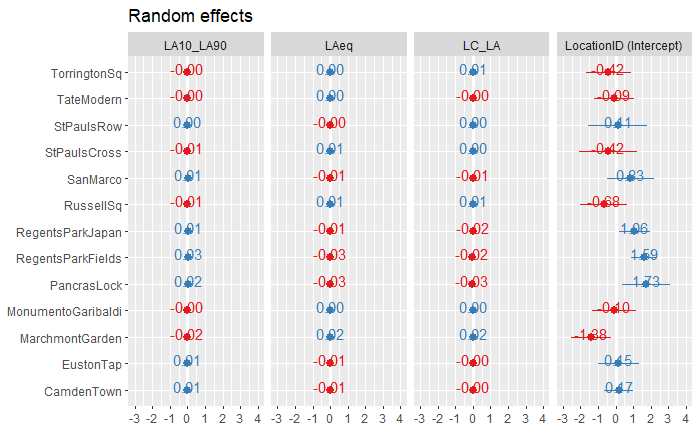
\includegraphics[width=\textwidth]{Figures/Lockdown Figure7.jpg}
    \caption{Unscaled location-level coefficients for the ISOPleasant model.}
    \label{fig:unsclRandom}
\end{figure}
